\documentclass[11pt,a4paper]{article}

\usepackage{natbib}
\usepackage{graphicx}
\usepackage{hyperref}
\graphicspath{ {./img/} }

\begin{document}
\title{chizuru4rogue: Deep Reinforcement Learning for Dungeon Crawling \\[1ex] \large Project Proposal}
\author{Dylan G. Drescher}
\date{November 2022}
\maketitle

\section{Problem Description}
\subsection{Introduction}
Rogue is a computer game that belongs to a genre called ``roguelikes". Roguelikes are a genre of computer game characterised by challenging, turn based dungeon crawling gameplay, procedurally generated levels and permanent character death. They are a fascinating domain to apply reinforcement learning methods to due to the amount of strategies and gameplay styles that roguelike games allow. Additionally, an agent playing a roguelike game would only need to perform one action per turn, and often times turns in these games are resolved near-instantly, allowing for efficient simulation and training.

The aim of chizuru4rogue is to apply deep reinforcement learning methods for an agent to learn, survive and thrive within Rogue. Reinforcement learning methods are suitable for this problem domain because they work well with games, due to the nature of games granting rewards for skilled play. The hope is that by the end of project development, chizuru4rogue will be able to play the game to a level where it can win the game, however further investigation into which methods are most suitable to accomplish this task will be performed during research and design of the agent, starting with researching methods used in other agents that play games such as AlphaGo.

Should the project prove successful, it can be used as a foundation for creating agents to play more complex roguelike games, such as NetHack or Cogmind, improving upon the program to allow the agent to adapt to these more complex environments.

\subsection{Problem Environment}
The environment the agent will interact with is the computer game Rogue, a 1980 terminal-based dungeon crawler and the namesake of the ``roguelike" genre, inspiring games similar to Rogue such as NetHack and Angband.
I am using Rogue as an environment as Rogue is a simpler game than its successors, while still being challenging enough to be an interesting problem to work with.

In Rogue, the player's objective is to navigate their way down numerous levels of a procedurally generated dungeon in order to reach the 26th level and collect the ``Amulet of Yendor".

The dungeon's layout is initially unknown, being revealed to the player as they explore. As the player explores the dungeon, the player will find items to loot and monsters to fight. If the player is killed, the game ends and the player must start from dungeon level 1. The player is given a score once the game ends.

\begin{figure}[t]
	\caption{A screenshot of an example Rogue game. Items, monsters and other map information are represented with a unique letter. Here, gold is represented with ``*", a kestrel enemy is represented with ``K" and the player character is represented with ``@".}
	\centering
	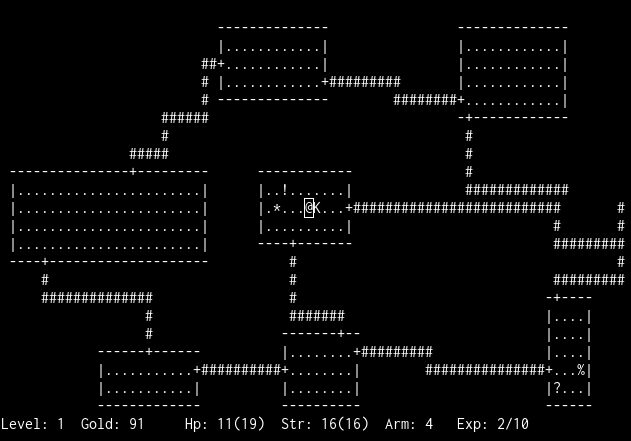
\includegraphics[scale=0.5]{rogue_screenshot}
	\label{rogsc}
\end{figure}

\subsection{Existing Systems}
There have been several attempts at creating an agent to play Rogue. One of the most prolific is Rog-O-Matic, an expert system developed in 1983 in Carnegie Mellon University that was observed to play as well as human players \cite[p.8]{mauldin83}. This system makes no use of any reinforcement learning methods, but provides a good yardstick for measuring how the agent should perform once it has been trained to play Rogue effectively.

Another, more recent attempt is Rogueinabox, a framework for Rogue agents where a Deep Q-Learning neural network was applied \cite[p.149]{asperti17}. Rogueinabox in their experiment lacked several core gameplay features that their agent could have considered such as combat and item usage, instead focusing on exploration without fighting enemies or collecting items.

While this is fine for testing an agent interacting within Rogue, the agent would need to be able to interact with the environment fully if the agent is to win the game, since if the agent never engages in combat with enemies, or collects better equipment, the agent will not get stronger, and will be easily killed by the later levels' enemies.

\section{Objectives}
\begin{enumerate}
	\item The first objective is to create a module that acts as an interface between Rogue and chizuru4rogue. It will take actions that the agent wishes to perform, runs that action in Rogue, takes the resulting consequence and encapsulate it in a way that chizuru4rogue can interpret.
	\item The second objective is to develop chizuru4rogue proper. During development, bug fixing will be common. The end goal of this stage is to get the agent created, running and learning.
	\item Once chizuru4rogue is in a working state, the third objective is to run chizuru4rogue over many episodes and measure its performance as it plays in terms of its final score.
	\item The fourth objective is to evaluate the data generated by the agent, summarise what has happened within the report, consider any improvements that could have been made during development and present other improvements for related future projects.
\end{enumerate}

\section{Requirements Specification}
\subsection{Interface Requirements}
\begin{enumerate}
	\item The interface must allow the agent to send an input to Rogue.
	\item The interface must be able to interpret Rogue's output.
	\item The interface must encapsulate Rogue's output so that it can be interpreted by the agent.
	\item The interface must tell the agent what actions it can currently take.
\end{enumerate}

\subsection{Agent Requirements}
\begin{enumerate}
	\item The agent must learn from its gameplay experiences.
	\item The agent must be able to interact with the game through the interface.
	\item The agent must perform some action during its turn.
	\item The agent must perform an action out of the action set that the interface gives.
	\item The agent must take the Rogue output and use it to learn from what has happened.
	\item The agent should improve its skill over many gameplay episodes.
	\item The agent could utilise LSTM
\end{enumerate}

\subsection{Project Requirements}
\begin{enumerate}
	\item The entire project must be complete and in a working state by the 1st May 2023.
	\item The project must have a Literature, Technology and Data Survey submitted by the 2nd December 2022.
	\item The project must have a Demonstration of Progress submitted by the 20th February 2023.
	\item The project should have a minimum viable product ready by the 20th February 2023.
\end{enumerate}

\section{System Plan}
\subsection{Plan Overview}
While Rogue is written in C, chizuru4rogue will be written in Python. The agent will not need to interact with the code of the game, it will only be able to use the same information that the game would give a human player. Python was chosen due to the large amount of machine-learning based libraries available for the language, such as TensorFlow.
An interface for Rogue will be created before work on the actual agent begins, also written in Python. This interface will allow chizuru4rogue to interact with Rogue, and it will send information back to the agent about the current state of the game, as well as any results due to the agent's actions.

The entire project's code will be managed on a Git repository, hosted on the online service \href{https://sourcehut.org}{Sourcehut}.

\subsection{Gantt Chart}
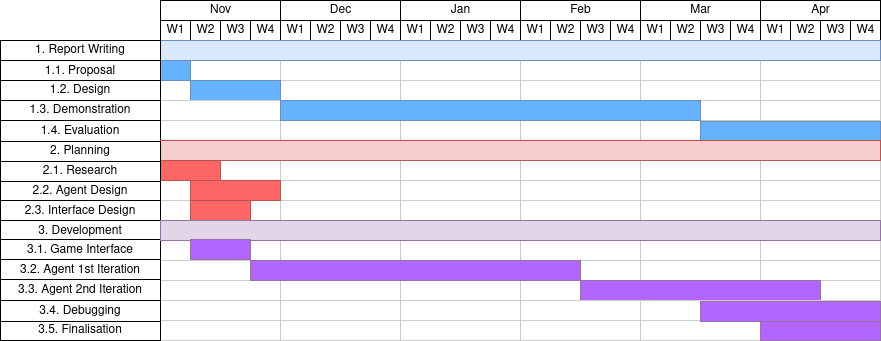
\includegraphics[scale=0.40]{ga}

\subsection{Required Resources}
Many reinforcement learning-based articles and books are available online, either for free or accessible through the university library, therefore no special provisions must be met in order to accomplish research and design.

Running reinforcement learning programs require lots of compute resources. To accomplish this project, I will need to contact the HPC departmental champion, James Davenport, to be granted access the University's Balena supercomputing environments.

\medskip

\bibliographystyle{agsm}
\bibliography{proposal}

\end{document}
